\newpage
\section{Xử lý dữ liệu}

\subsection{Tải dữ liệu và tổng quan về dữ liệu} 
\paragraph{}{Dữ liệu phục vụ huấn luyện mô hình được cung cấp trong file \texttt{train.csv}, trong đó bao gồm:}
\begin{itemize}
    \item \textbf{1647 dòng}, cung cấp chi tiết về thông số kỹ thuật, đặc điểm và giá của các loại xe ô tô.
    \item \textbf{20 cột} dữ liệu, trong đó có 8 cột chứa dữ liệu số, 12 cột chứa dữ liệu chữ: 
    \begin{itemize}
        \item \texttt{Make}, \texttt{Model}: Hãng sản xuất xe, tên mẫu xe cụ thể.
        \item \texttt{Price}: Giá niêm yết hoặc giá bán của xe.
        \item \texttt{Year}: Năm sản xuất của xe.
        \item \texttt{Kilometer}: Tổng số kilomet xe đã di chuyển.
        \item \texttt{Fuel Type}: Loại nhiên liệu xe sử dụng (ví dụ: Xăng, Dầu Diesel, Điện).
        \item \texttt{Transmission}: Loại hộp số (ví dụ: Số sàn, Số tự động).
        \item \texttt{Location}: Địa điểm, thành phố hoặc khu vực bán xe.
        \item \texttt{Color}: Màu sơn ngoại thất của xe.
        \item \texttt{Owner}: Số lượng chủ sở hữu trước đây của xe.
        \item \texttt{Seller Type}: Loại hình người bán (ví dụ: Cá nhân, Đại lý).
        \item \texttt{Engine}: Dung tích xi-lanh của động cơ, thường tính bằng cc (cubic centimeters).
        \item \texttt{Max Power}: Công suất cực đại mà động cơ có thể tạo ra (bhp - brake horsepower).
        \item \texttt{Max Torque}: Mô-men xoắn cực đại mà động cơ có thể tạo ra (Nm - Newton-meters).
        \item \texttt{Drivetrain}: Hệ thống truyền động lực từ động cơ đến bánh xe 
        \item \texttt{Length}, \texttt{Width}, \texttt{Height}: Chiều dài, chiều rộng, chiều cao tổng thể của xe (mm).
        \item \texttt{Seating Capacity}: Số lượng chỗ ngồi tối đa trong xe (bao gồm cả lái xe).
        \item \texttt{Fuel Tank Capacity}: Dung tích tối đa của bình chứa nhiên liệu, tính bằng lít.
    \end{itemize}
    \item 149 dòng có chứa dữ liệu NaN (Not a Number).
\end{itemize}

\begin{figure}[H]
    \centering
    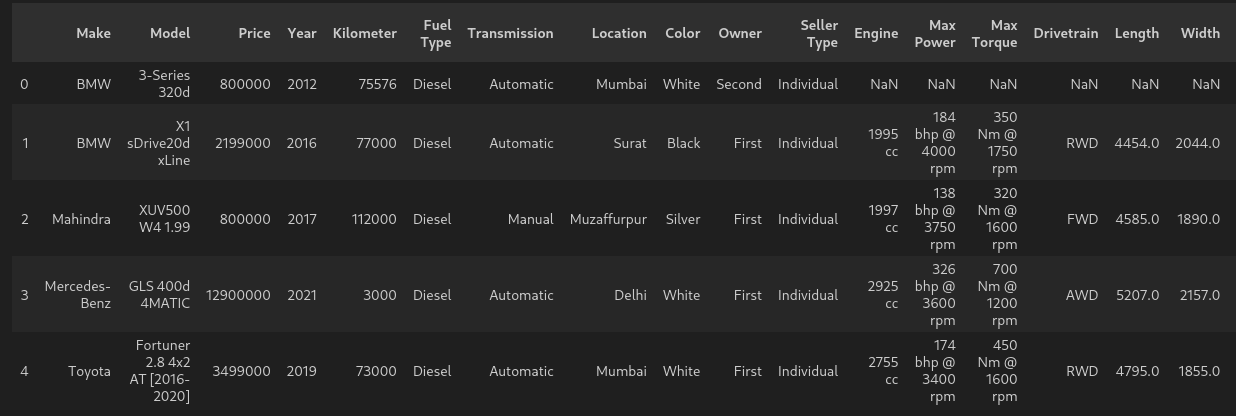
\includegraphics[width=1\linewidth]{img/data-head.png}
    \caption{Các dòng đầu tiên trong bộ dữ liệu}
    \label{fig:data-head}
\end{figure}

\subsection{Tiền xử lý dữ liệu - Data preprocessing}

\subsubsection{Chia tập dữ liệu huấn luyện - kiểm chứng}

\paragraph{}{Khi xử lí dữ liệu đầu vào, các bước như làm sạch dữ liệu và mã hóa dữ liệu sẽ lấy thông tin của tổng thể như trung vị (median), giá trị có tần suất xuất hiện lớn nhất để điền vào các dòng bị thiếu thông tin. Vì vậy, để tránh hiện tượng \textbf{rò rỉ thông tin} (data leakage), ta cần chia tập dữ liệu thành \textbf{tập huấn luyện} (training set) và \textbf{tập kiểm chứng} (validation set) ngay trước khi xử lí dữ liệu.}

\paragraph{}{Chia tập dữ liệu thành \textbf{tập huấn luyện} và \textbf{tập kiểm chứng} giúp ta đánh giá mô hình chính xác hơn, giúp nhận biết tốt hiện tượng \textbf{quá khớp} (overfitting) hoặc \textbf{dưới khớp} (underfitting).}

\paragraph{}{Tập huấn luyện và tập kiểm chứng được chia với tỉ lệ lần lượt là 0.8 và 0.2 so với tổng dữ liệu.}

\subsubsection{Làm sạch dữ liệu}
\paragraph{}{Ở bước làm sạch dữ liệu (Data cleaning), có 3 kĩ thuật chính được sử dụng:}

\begin{itemize}
    \item Điền vào ô NaN ở các cột có đặc trưng số với giá trị trung bình của chúng.
    \item Điền vào ô NaN ở các cột có đặc trưng phi số với giá trị xuất hiện thường xuyên nhất.
    \item Xóa các dòng dữ liệu lặp.
\end{itemize}

\paragraph{}{Tập kiểm chứng sẽ được điền vào ô NaN dựa trên thông tin (giá trị trung bình, giá trị xuất hiện thường xuyên nhất) lấy được từ tập huấn luyện.}

\subsubsection{Chuyển đổi dữ liệu}

\paragraph{}{Ở bước chuyển đổi dữ liệu (Data transformation), có 3 bước:}

\begin{itemize}
    \item Thêm các cột dữ liệu: \texttt{rpm at Max Power} (vòng tua tại công suất cực đại) và \texttt{rpm at Max Torque} (vòng tua tại Mô-men xoắn cực đại). 
    \item Cột dữ liệu \texttt{Max Power} và \texttt{Max Torque} được biến đổi, không còn các dữ liệu về vòng tua do đã được tách ra thành cột riêng.
    \item Các cột có đặc trưng số sẽ được đưa về dạng dữ liệu \texttt{int} (số nguyên).
\end{itemize}

\newpage
\subsection{Trực quan hóa dữ liệu - Data visualization}

\paragraph{}{Sau đây là một vài biểu đồ thể hiện chi tiết dữ liệu (trên tập train):}

\subsubsection{Ma trận tương quan của các đặc trưng số}
\begin{figure}[H]
    \centering
    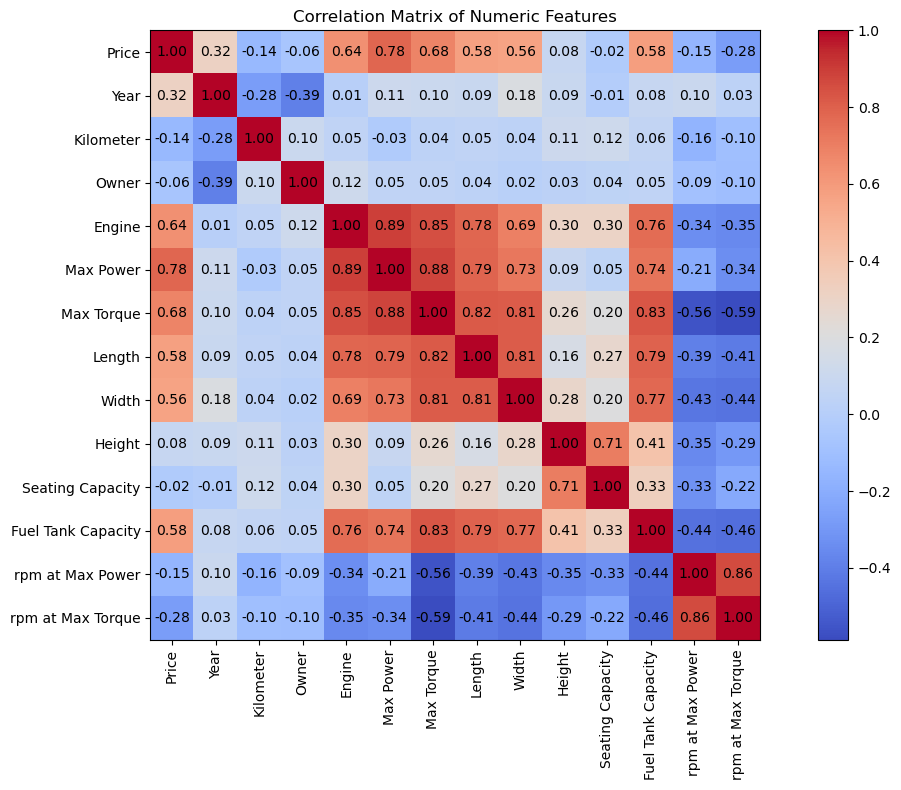
\includegraphics[width=1\linewidth]{img/corr-matrix-1.png}
    \caption{Ma trận tương quan}
    \label{fig:corr-matrix-1}
\end{figure}

\subsubsection{Biểu đồ Histogram của các đặc trưng số}
\begin{figure}[H]
    \centering
    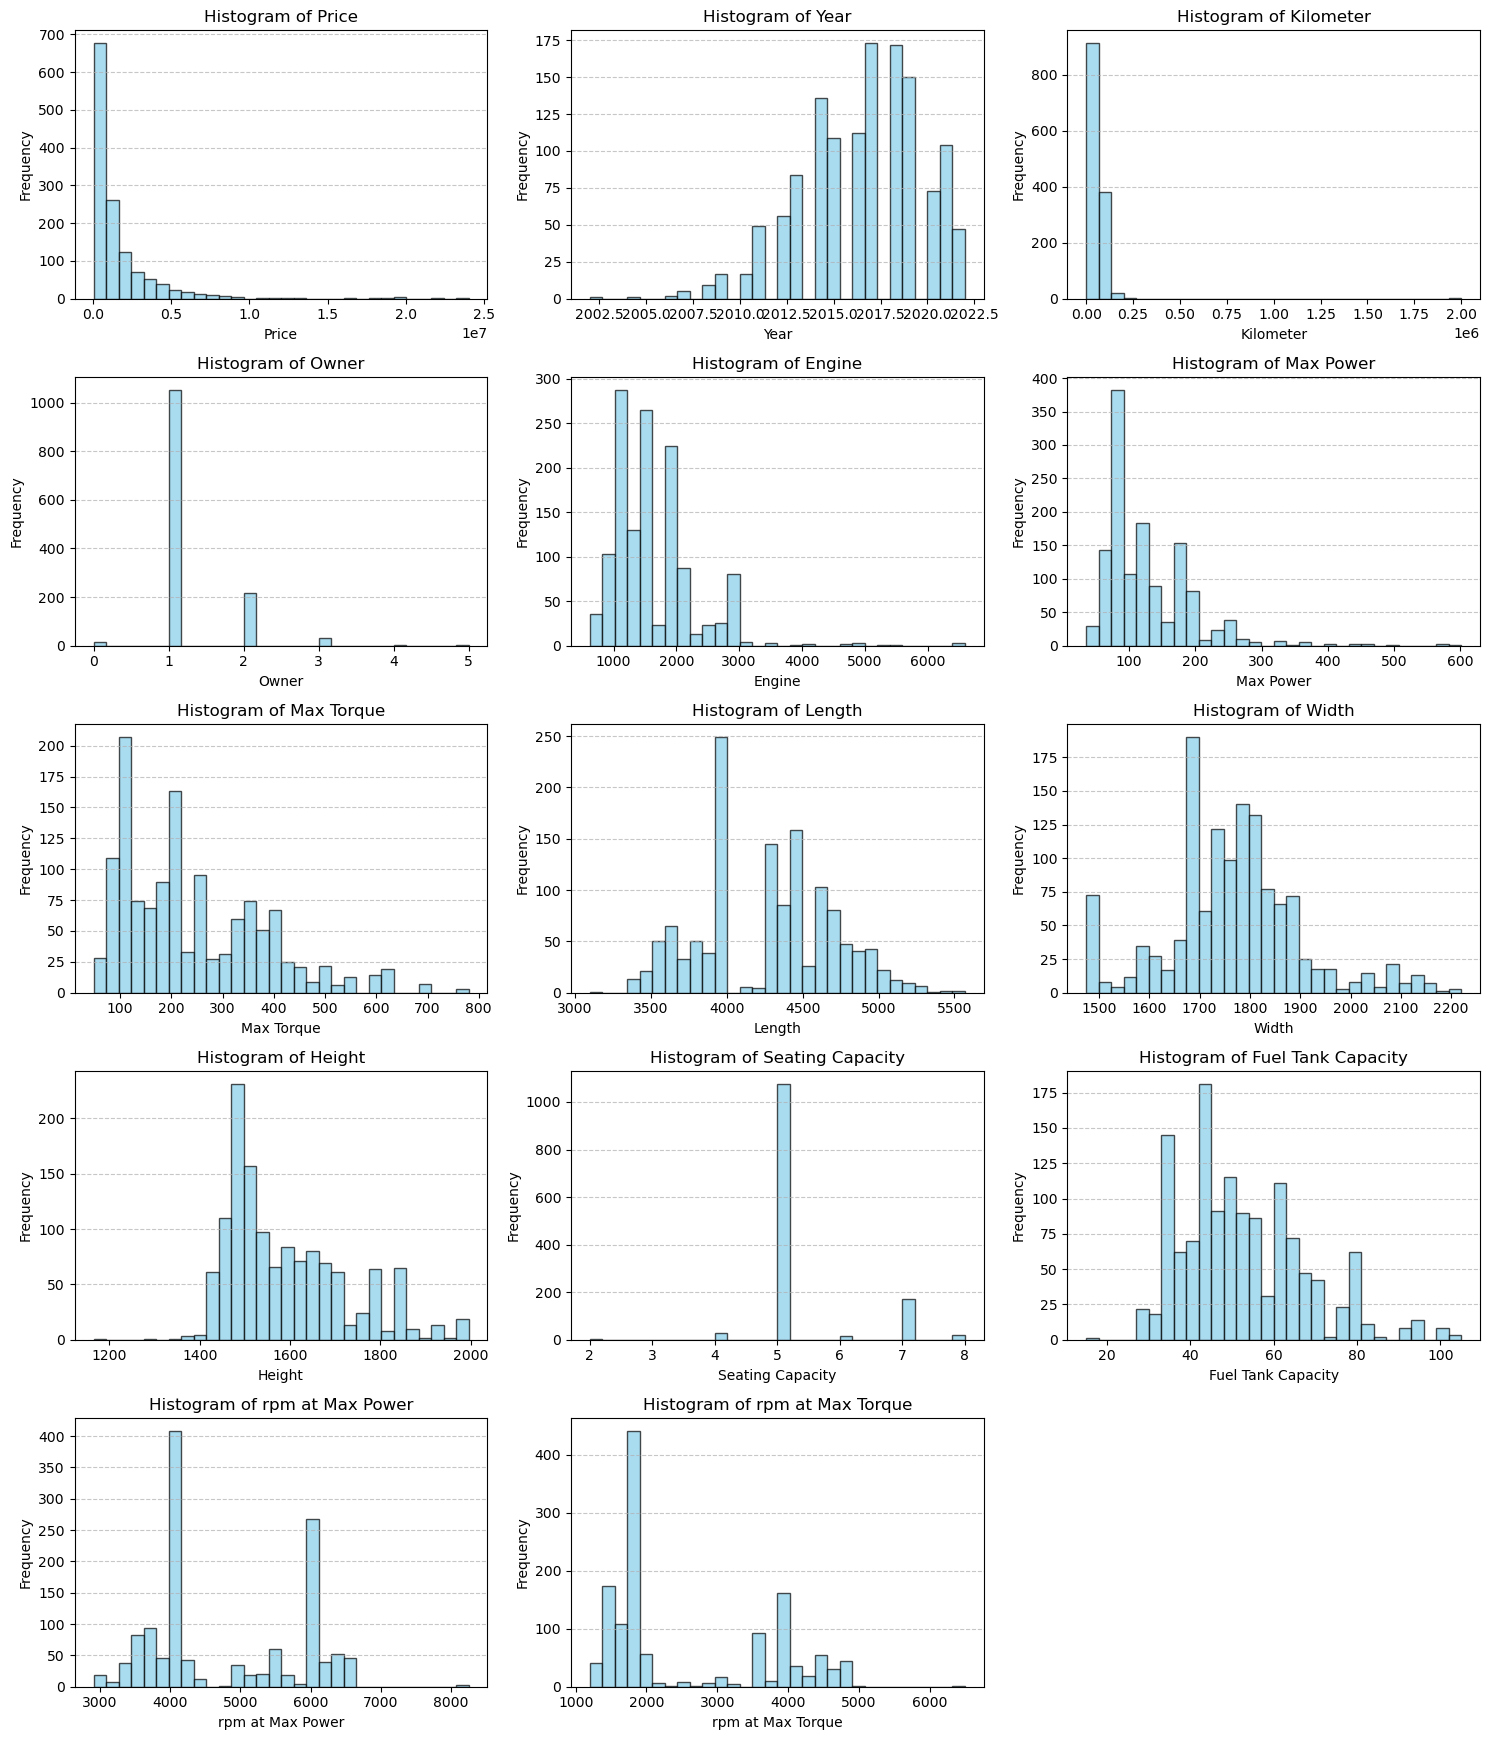
\includegraphics[width=1\linewidth]{img/histogram-1.png}
    \caption{Biểu đồ Histogram của các đặc trưng số}
    \label{fig:histogram-1}
\end{figure}

\subsubsection{Biểu đồ phân tán của các đặc trưng số}
\begin{figure}[H]
    \centering
    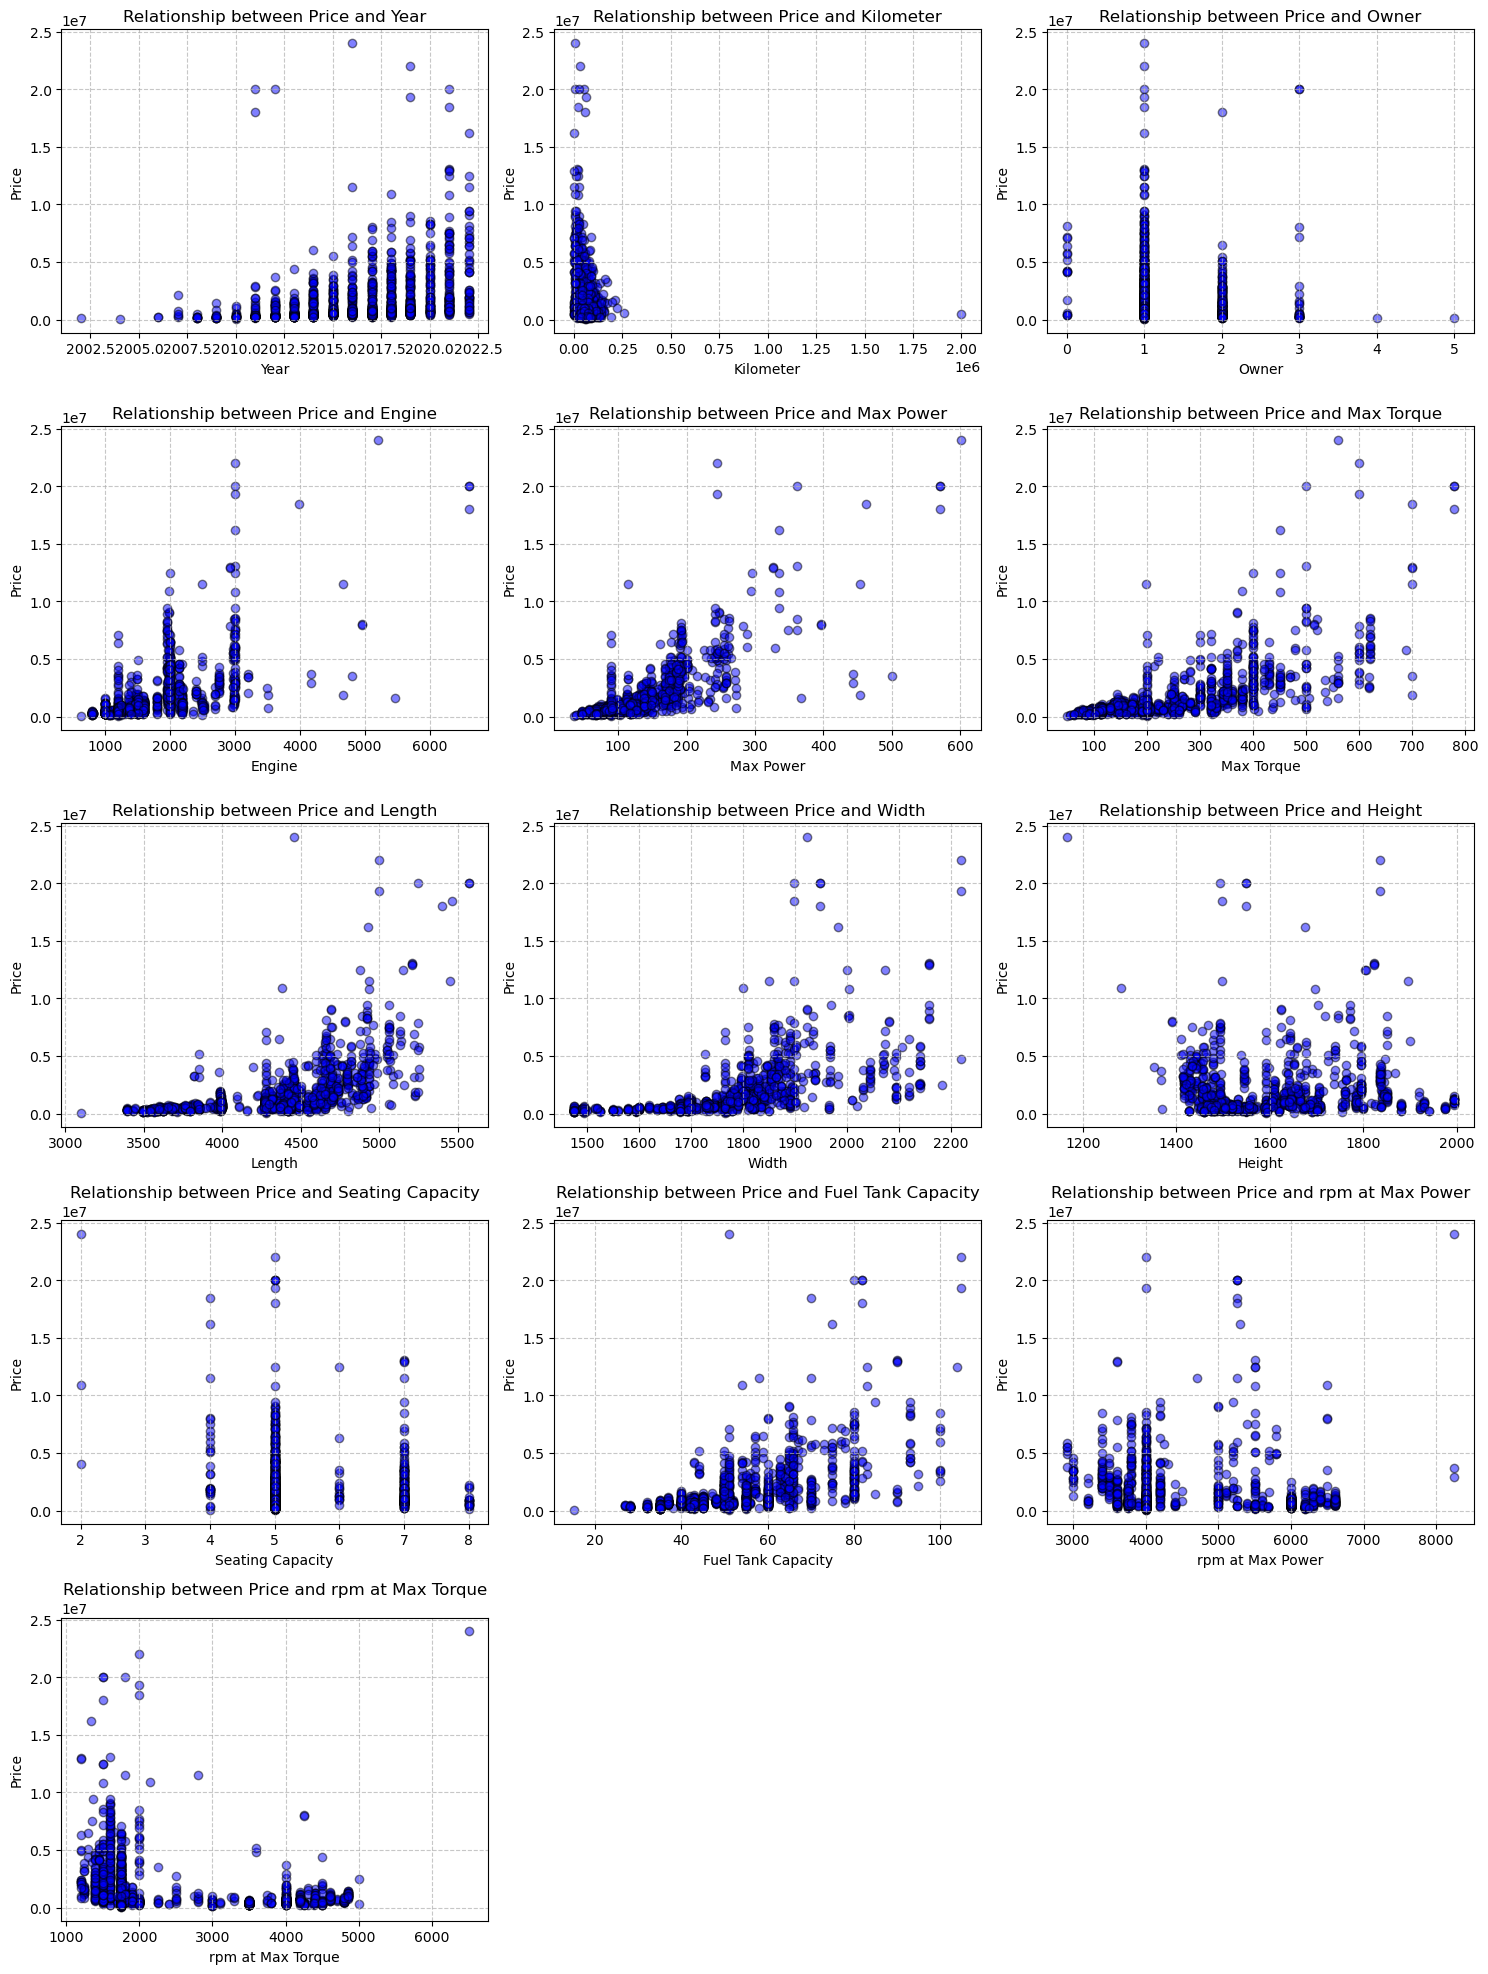
\includegraphics[width=0.9\linewidth]{img/scatter-plot.png}
    \caption{Biểu đồ phân tán so sánh giá xe theo các đặc trưng số}
    \label{fig:scatter-plot}
\end{figure}

\subsubsection{Biểu đồ hộp của các đặc trưng phi số}
\begin{figure}[H]
    \centering
    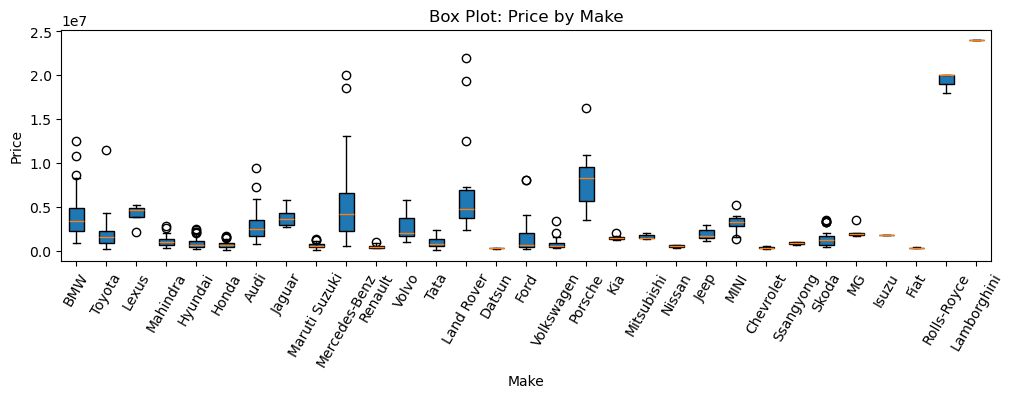
\includegraphics[width=1\linewidth]{img/boxplot-make.png}
    \caption{Biểu đồ hộp so sánh giá xe theo hãng (Make)}
    \label{fig:boxplot-make}
\end{figure}

\begin{figure}[H]
    \centering
    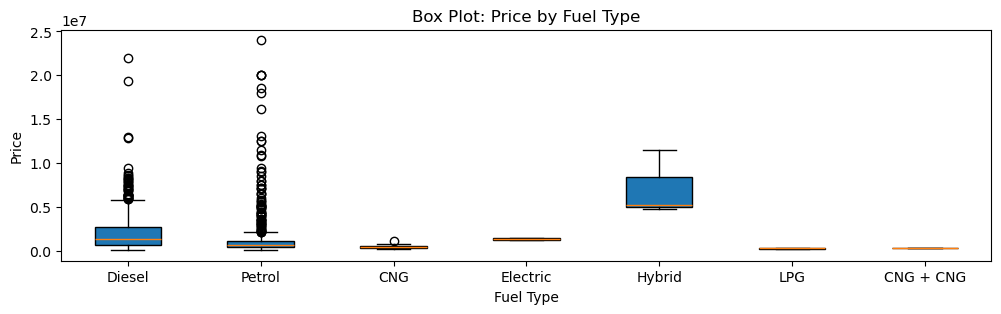
\includegraphics[width=1\linewidth]{img/boxplot-fueltype.png}
    \caption{Biểu đồ hộp so sánh giá xe theo loại nhiên liệu sử dụng (Fuel Type)}
    \label{fig:boxplot-fueltype}
\end{figure}

\begin{figure}[H]
    \centering
    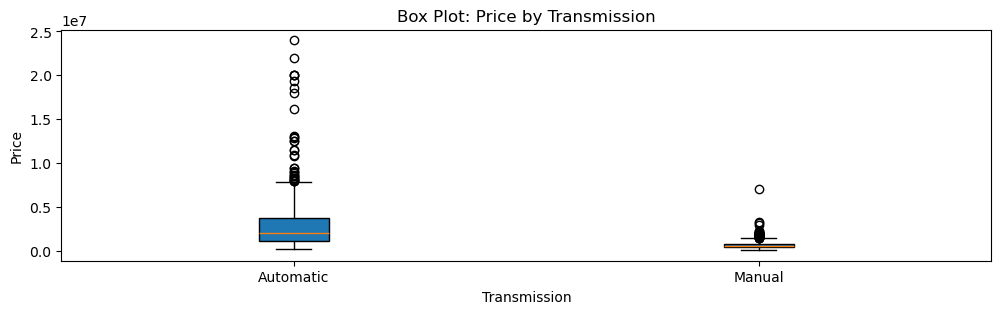
\includegraphics[width=1\linewidth]{img/boxplot-transmission.png}
    \caption{Biểu đồ hộp so sánh giá xe theo loại hộp số (Transmission)}
    \label{fig:boxplot-transmission}
\end{figure}

\begin{figure}[H]
    \centering
    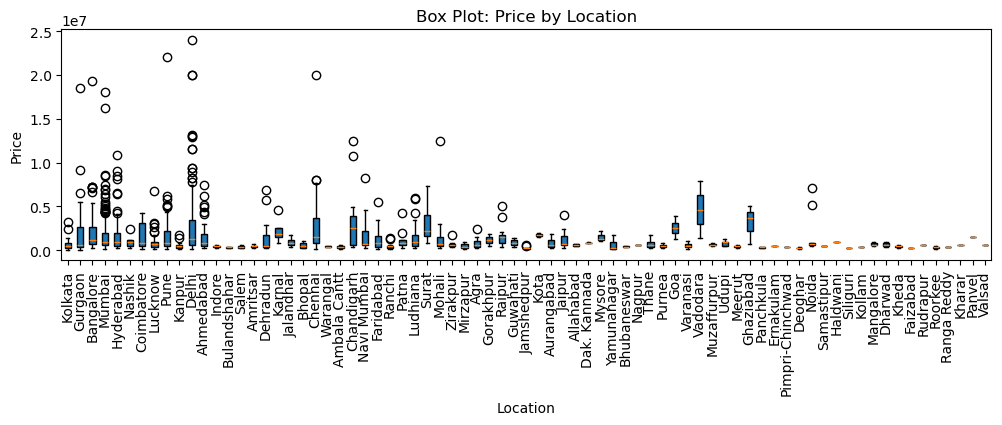
\includegraphics[width=1\linewidth]{img/boxplot-location.png}
    \caption{Biểu đồ hộp so sánh giá xe theo địa điểm (Location)}
    \label{fig:boxplot-location}
\end{figure}

\begin{figure}[H]
    \centering
    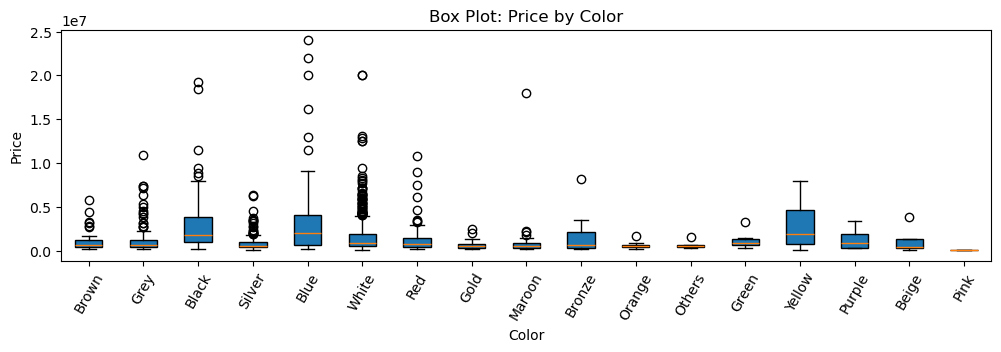
\includegraphics[width=1\linewidth]{img/boxplot-color.png}
    \caption{Biểu đồ hộp so sánh giá xe theo màu sắc (Color)}
    \label{fig:boxplot-color}
\end{figure}

\begin{figure}[H]
    \centering
    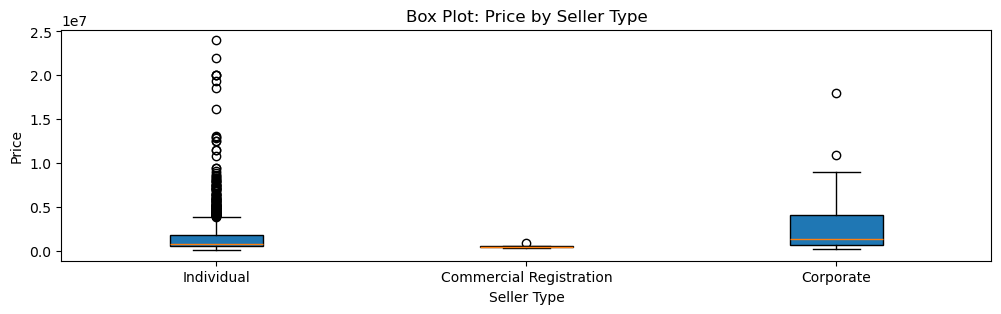
\includegraphics[width=1\linewidth]{img/boxplot-sellertype.png}
    \caption{Biểu đồ hộp so sánh giá xe theo loại người bán (Seller type)}
    \label{fig:boxplot-sellertype}
\end{figure}

\begin{figure}[H]
    \centering
    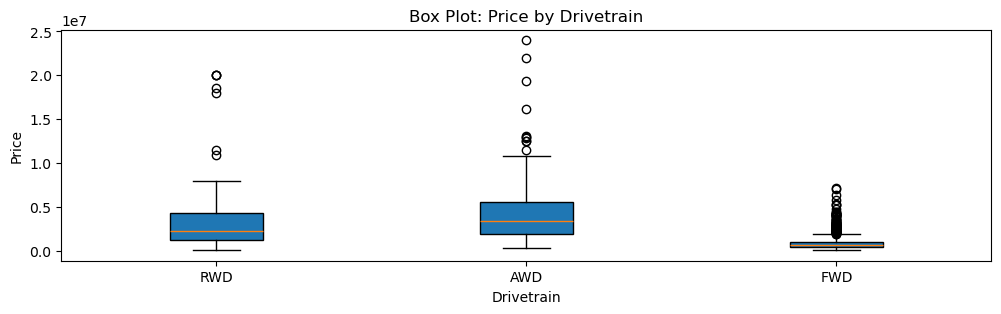
\includegraphics[width=1\linewidth]{img/boxplot-drivetrain.png}
    \caption{Biểu đồ hộp so sánh giá xe theo loại hệ dẫn động (Drivetrain)}
    \label{fig:boxplot-drivetrain}
\end{figure}

\subsubsection{Kết luận}
\paragraph{}{Từ dữ liệu được trực quan hóa, ta rút ra được một số nhận xét sau:}

\begin{itemize}
    \item Phân bố giá trị của các đặc trưng số là gần theo \textbf{phân phối chuẩn}. Ngoài ra đặc trưng giá xe (Price) và số kilomet đi được (Kilometer) lệch phải nặng (hình \ref{fig:histogram-1}). 
    \item Các đặc trưng phi số có thể được \textbf{mã hóa} thành các \textbf{đặc trưng số}.
    \item \textbf{Khoảng giá trị} của mỗi đặc trưng số là \textbf{rất khác nhau}, hoặc là rất to, hoặc là rất nhỏ. Dữ liệu cần được chuẩn hóa để giúp mô hình học tốt hơn\footnote{Xem chứng minh ở phần cơ sở toán học}.
    \item Giá xe có sự khác biệt đáng kể giữa các \textbf{hãng} và các \textbf{mẫu xe} khác nhau (hình \ref{fig:boxplot-make}), ta có thể thay thế mỗi hãng và mẫu xe bằng \textbf{giá trị trung vị} tương ứng của các xe thuộc hãng/mẫu.
    \item Giá xe Hybrid \textbf{cao hơn}\footnote{Có giá trị trung vị cao hơn và khoảng IQR đủ nhỏ} so với các loại xe sử dụng nhiên liệu khác (hình \ref{fig:boxplot-fueltype}). Tương tự, số sàn cao hơn số tự động (hình \ref{fig:boxplot-transmission}); các địa điểm bán cao hơn trung vị nhìn chung cao hơn các địa điểm còn lại (hình \ref{fig:boxplot-location}); màu đen, xanh dương và vàng cao hơn các màu khác (hình \ref{fig:boxplot-color}); công ty cao hơn cá nhân và đại lý (hình \ref{fig:boxplot-sellertype}); hệ dẫn động AWD cao hơn RWD và RWD cao hơn FWD (hình \ref{fig:boxplot-drivetrain}). Các nhận định này giúp ta \textbf{mã hóa nhị phân} (loại nhiên liệu, hộp số, địa điểm bán, màu sắc, người bán) hoặc \textbf{mã hóa theo thứ tự giá trị} (hệ dẫn động) các đặc trưng phi số, giúp mô hình học một cách hiệu quả.
\end{itemize}

\subsection{Mã hóa dữ liệu - Data encoding}
\paragraph{}{Từ những kết luận rút ra từ việc trực quan hóa dữ liệu, ta sẽ mã hóa các đặc trưng phi số về đặc trưng số. Điều này giúp tăng các đặc trưng mà mô hình có thể học.}

\begin{itemize}
    \item \textbf{Hãng xe} (Make): Thay bằng giá trung vị của các xe thuộc hãng đó.
    \item \textbf{Mẫu xe} (Model): Thay bằng giá trung vị của các xe cùng mẫu.
    \item \textbf{Loại nhiên liệu} (Fuel Type): Xe Hybrid thay bằng 1, các loại xe còn lại thay bằng 0.
    \item \textbf{Hộp số} (Transmission): Xe có hộp số tự động (Auto) thay bằng 1, hộp số sàn (Manual) thay bằng 0.
    \item \textbf{Địa điểm} (Location): Nếu giá trung vị của các xe có cùng địa điểm lớn hơn hoặc bằng giá trung vị toàn cục thì thay bằng 1; ngược lại thay bằng 0.
    \item \textbf{Màu sắc} (Color): Xe có màu trắng, xanh dương hoặc vàng thì thay bằng 1, còn lại là 0.
    \item \textbf{Loại người bán} (Seller Type): Nếu xe được bán bởi các công ty (Corporate) thì thay bằng 1, còn lại là 0.
    \item \textbf{Hệ dẫn động} (Drivetrain): FWD thay bằng 1, RWD thay bằng 2, AWD thay bằng 3.
\end{itemize}

\paragraph{}{Sau khi mã hóa các dữ liệu, ta có tổng cộng 23 đặc trưng số và không còn đặc trưng phi số.}

\subsection{Chuẩn hóa dữ liệu - Data normalization}

\paragraph{}{Từ những kết luận rút ra từ việc trực quan hóa dữ liệu, ta nhận thấy khoảng giá trị của mỗi đặc trưng số là rất khác nhau. Chẳng hạn, sức chứa chỗ ngồi (Seating capacity) nằm trong khoảng $[2, 8]$ còn công suất tối đa (Max power) nằm trong khoảng $[3000, 8000]$ (hình \ref{fig:histogram-1}). Điều đó dẫn đến một việc tất yếu là phải \textbf{chuẩn hóa dữ liệu} về một khoảng giá trị, giúp mô hình học và dự đoán tốt hơn.}

\subsubsection{Phương pháp chuẩn hóa dữ liệu}
\paragraph{}{Từ hình \ref{fig:histogram-1}, ta có nhận xét: phân phối của các đặc trưng nhìn chung tuân theo phân phối chuẩn, đặc trưng \texttt{Kilometer} có phân phối bị lệch phải. Ta sẽ áp dụng $log(x+1)$ Transformation \cite{benoit2011linear} cho \texttt{Kilometer}, sau đó áp dụng MinMax Scaler, Standard Scaler \cite{brownlee2020use} cho tất cả các đặc trưng.}
\begin{enumerate}
    \item \textbf{Log(x+1) Transformation} được sử dụng để xử lý dữ liệu bị lệch (skewed), làm cho phân phối gần với phân phối chuẩn hơn. Việc sử dụng $log(x+1)$ thay vì $log(x)$ giúp xử lý các giá trị bằng 0.

    \begin{center}
    \large $x_{scaled} = \log(x+1)$
    \end{center}

    Trong đó:
    \begin{itemize}
        \item $x_{scaled}$: Giá trị đã được chuẩn hóa.
        \item $x$: Giá trị ban đầu.
    \end{itemize}

    \item \textbf{MinMax Scaler} co giãn các giá trị về một phạm vi cụ thể, thường là từ 0 đến 1.

    \begin{center}
    \large $x_{scaled} = \frac{x - \min(x)}{\max(x) - \min(x)}$
    \end{center}

    Trong đó:
    \begin{itemize}
        \item $x_{scaled}$: Giá trị đã được chuẩn hóa.
        \item $x$: Giá trị ban đầu.
        \item $\min(x)$: Giá trị nhỏ nhất của đặc trưng trong tập dữ liệu.
        \item $\max(x)$: Giá trị lớn nhất của đặc trưng trong tập dữ liệu.
    \end{itemize}

    \item \textbf{Standard Scaler (Chuẩn hóa Z-score)} (xem \ref{label:standart scaler}) được dùng cho phương pháp PCA.
\end{enumerate}

\subsubsection{Ma trận tương quan sau mã hóa và chuẩn hóa}

\begin{figure}[H]
    \centering
    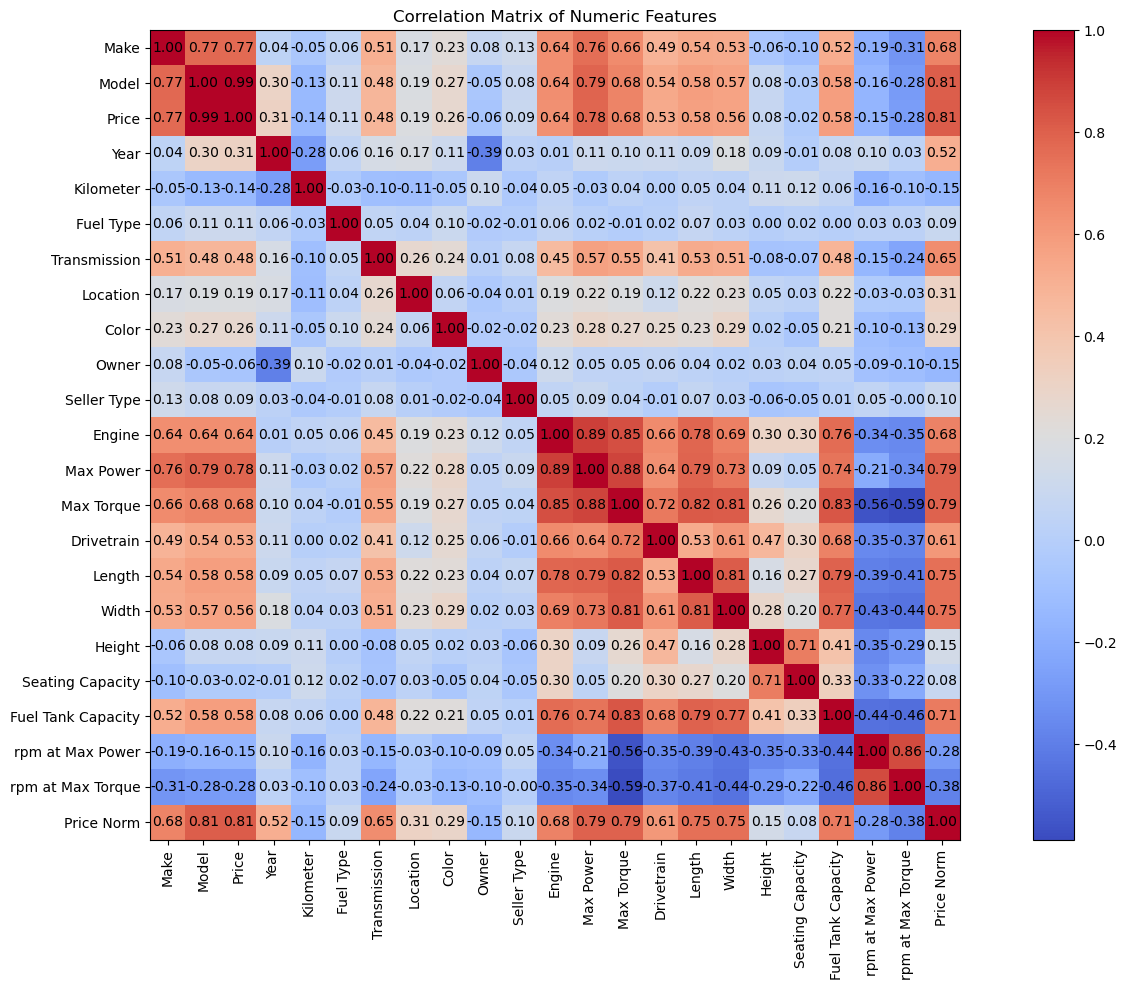
\includegraphics[width=1\linewidth]{img/corr-matrix-2.png}
    \caption{Ma trận tương quan sau khi mã hóa và chuẩn hóa dữ liệu}
    \label{fig:corr-matrix-2}
\end{figure}

\paragraph{Nhận xét:}{Sau khi mã hóa và chuẩn hóa dữ liệu, ta thấy đặc trưng \texttt{Model} có sự tương quan lớn với \texttt{Price}. Đây sẽ là cơ sở để lựa chọn đặc trưng, phục vụ các mô hình hồi quy (đặc biệt là mô hình hồi quy tuyến tính đơn).}

\pagebreak